\nte[Section 2.2]{Oct 14 2024 Mon (13:00:26)}{Limit of a Sequence}

\section{Required Definitions}
\label{sec:required_definitions}

\begin{definition}
  A \textit{sequence} is a function whose domain is $\N$.
\end{definition}

Given a function $f : \N \to \R$, $f(n)$ is just the $n$th term on the list.

\begin{example}
  Each of the following are common ways to describe sequences.
  \begin{enumerate}
    \item $(1, \frac{1}{2}, \frac{1}{3}, \frac{1}{4}, \dots)$.

    \item $(\frac{1 + n}{n})_{n=1}^{\infty} = (\frac{2}{1}, \frac{3}{2},
      \frac{4}{5}, \dots)$.

    \item $(a_n)$, where $a_n = 2^n$ for each $n \in \N$.

    \item $(x_n)$, where $x_1 = 2$ and $x_{n+1} = \frac{x_n + 1}{2}$.
  \end{enumerate}
\end{example}

\begin{definition}[Convergence of a Sequence]
  A sequence $(a_n)$ \textit{converges} to a real number $\ell$ if,
  \[%
    (\forall \epsilon > 0)(\exists N \in \N)(\forall n \ge N) \lvert a_n - \ell \rvert < \epsilon
  .\]%
  We say that $\ell$ is the limit of $(a_n)$.
\end{definition}

One way to think of $(\exists N \in \N)(\forall n \ge N)$ as saying ``eventually
always'', or as ``from some point on''. So, the definition means, if $a_n \to
\ell$, then given any $\epsilon$, then eventually, everything in the sequence is
within $\epsilon$ of $\ell$. You may know this as $\lim_{n \to \infty} a_n = a$.
This is a more formal definition of the limit of a sequence.

\begin{definition}
  Given a real number $a \in \R$ and an $\epsilon > 0$, the set
  \[%
    V_{\epsilon} (a) = \{x \in \R \mid \lvert x - a \rvert < \epsilon\}
  ,\]%
  is called the \textit{$\epsilon$-neighborhood} of $a$.
\end{definition}

The $V_{\epsilon}(a)$ is just an interval centered at $a$ with radius
$\epsilon$.
\begin{figure}[H]
  \centering

  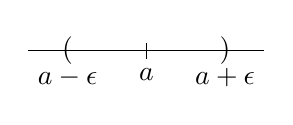
\begin{tikzpicture}
    \draw (-1.5, 0) -- (1.5, 0);

    \node[below=3pt] at (-1, 0) {$a - \epsilon$};
    \node at (-1, 0) {$($};

    \node[midway,below=3pt] at (0, 0) {$a$};
    \draw (0, 0.1) -- (0, -0.1);

    \node[below=3pt] at (1, 0) {$a + \epsilon$};
    \node at (1, 0) {$)$};
  \end{tikzpicture}
\end{figure}

Using the $V_{\epsilon}(a)$ definition, $(a_n)$ converges if, at a certain point
$k$, every term after $k$ is in the $\epsilon$-neighborhood of $a$.

We can re-write the definition of convergence as follows using a topological
version instead of a more numerical analysis way as follows
\begin{definition}[Convergence of a Sequence: Topological Version]
  A sequence $(a_n)$ converges to $a$ if, given any $\epsilon$-neighborhood
  $V_{\epsilon}(a)$ of $a$, there exists a point in the sequence after which all
  of the terms are in $V_{\epsilon}(a)$. In other words, every
  $\epsilon$-neighborhood contains all but a finite number of the terms of
  $(a_n)$.
\end{definition}

\begin{figure}[H]
  \centering

  \begin{tikzpicture}
    \draw (-5, 0) -- (5, 0);

    \node[below=3pt] at (0, 0) {$a - \epsilon$};
    \node at (0, 0) {$($};

    \node[below=3pt] at (1.5, 0) {$a$};
    \draw (1.5, 0.1) -- (1.5, -0.1);

    \node[below=3pt] at (3, 0) {$a + \epsilon$};
    \node at (3, 0) {$)$};

    % Outside the interval
    \draw[soldot,above=5pt] (-4.5, 0) circle (2pt) node[above] {$a_1$};
    \draw[soldot,above=5pt] (-3.75, 0) circle (2pt) node[above] {$a_2$};
    \draw[soldot,above=5pt] (-3, 0) circle (2pt) node[above] {$a_3$};
    \draw[soldot,above=5pt] (-2.25, 0) circle (2pt) node[above] {$\cdots$};
    \draw[soldot,above=5pt] (-1.5, 0) circle (2pt);
    \draw[soldot,above=5pt] (-1, 0) circle (2pt);
    \draw[soldot,above=5pt] (-0.75, 0) circle (2pt);
    \draw[soldot,above=5pt] (-0.50, 0) circle (2pt);
    \draw[soldot,above=5pt] (-0.25, 0) circle (2pt);

    % Inside the interval
    \draw[soldot,above=5pt] (0.1, 0) circle (2pt);
    \draw[soldot,above=5pt] (0.3, 0) circle (2pt);
    \draw[soldot,above=5pt] (0.5, 0) circle (2pt);
    \draw[soldot,above=5pt] (0.7, 0) circle (2pt);
    \draw[soldot,above=5pt] (0.9, 0) circle (2pt);
    \draw[soldot,above=5pt] (1.1, 0) circle (2pt);
    \draw[soldot,above=5pt] (1.2, 0) circle (2pt);
    \draw[soldot,above=5pt] (1.3, 0) circle (2pt);
    \draw[soldot,above=5pt] (1.4, 0) circle (2pt);

    \draw[soldot,above=5pt] (1.6, 0) circle (2pt);
    \draw[soldot,above=5pt] (1.7, 0) circle (2pt);
    \draw[soldot,above=5pt] (1.8, 0) circle (2pt);
    \draw[soldot,above=5pt] (1.9, 0) circle (2pt);
    \draw[soldot,above=5pt] (2.1, 0) circle (2pt);
    \draw[soldot,above=5pt] (2.3, 0) circle (2pt);
    \draw[soldot,above=5pt] (2.5, 0) circle (2pt);
    \draw[soldot,above=5pt] (2.7, 0) circle (2pt);
    \draw[soldot,above=5pt] (2.9, 0) circle (2pt);

    \draw[decorate,decoration={brace,amplitude=5pt},thick] (0, 0.4) -- (3, 0.4) node[midway, above=5pt] {$V_{\epsilon}(a)$};
  \end{tikzpicture}
\end{figure}

Both definitions are equivalent. The topological version is more general and
applies to more than just sequences. It should be apparent that the value of $N$
depends on the choice of $\epsilon$. The smaller the $\epsilon$-neighborhood,
the larger $N$ may need to be.

% section required_definitions (end)

\section{Working with Limits}
\label{sec:working_with_limits}

\subsection{Quantifiers}
\label{sub_sec:quantifiers}

The definition begins with $(\forall \epsilon > 0)$. This means that we are
trying to prove that the sequence converges for all $\epsilon > 0$. Say,
$\epsilon = 0.00000001$, or $\epsilon = 100000000$, and so on.

The next quantifier is $(\exists N \in \N)$. This means that we need to find a
natural number $N$ such that the condition holds for all $n \ge N$. This doesn't
have to hold for all $N \in \N$, but just one specific value of $N$ will do,
which is typically the hardest part of the proof.

\begin{note}
  The order of the quantifiers is important. In the definition of convergence,
  we have $(\forall \epsilon > 0)(\exists N \in \N)$. This means that $N$ is
  dependent on $\epsilon$. If we had it the other way around, $(\exists N \in
  \N)(\forall \epsilon > 0)$, then we would have to find a single $N$ that works
  for all $\epsilon$, which is not possible.
\end{note}

Here's a template for a proof of $(x_n) \to x$.

\begin{proof} $ $
  \begin{itemize}
    \item ``Let $\epsilon > 0$ be arbitrarily chosen.''

    \item Demonstrate a choice for $N \in \N$. This is the hardest and most time
      consuming part of the proof.

    \item Now, show that $N$ actually works.

    \item ``Assume $n \ge N$.''

    \item You should be able to derive the inequality $\lvert x_n - x \rvert <
      \epsilon$, if your $N$ is chosen well enough. \qedhere
  \end{itemize}
\end{proof}

% subsection quantifiers (end)

\subsection{Examples}
\label{sub_sec:examples}

\begin{question}
  Prove that $(\frac{1}{\sqrt{n}}) \to 0$.
\end{question}

\begin{worksheet}
  Let's first explore the relationship between $\epsilon$ and $N$. Take
  $\epsilon = \sfrac{1}{10}$. This gives us a target zone for the terms in the
  sequence. By claiming that the limit of $(a_n)$ is $0$, we are saying that the
  terms in the sequence get arbitrarily close to $0$. But how close? This is
  where $\epsilon$ comes into play. We want to show that the terms in the
  sequence are within $\sfrac{1}{10}$ of $0$ after a certain point and they stay
  that way, if not get closer.
  The $100$th term $a_{100} = \sfrac{1}{10}$ puts us right on the boundary,
  giving us
  \[%
    \textrm{if}~n > 100, \qtq{then} a_n \in \left(-\frac{1}{10}, \frac{1}{10}\right)
  .\]%
  As you can see, the smaller we choose $\epsilon$, the larger we'll have to
  make $n$. Now, let's try and find $N$ for all $\epsilon > 0$.
  \begin{note}
    \textit{We aren't using a fixed $\epsilon$, since, say $\epsilon =
    \sfrac{1}{10}$, then $N > 100$, say $N = 101$, and were done, so that's just
    trivial}
  \end{note}
  We have the inequality
  \[%
    \frac{1}{\sqrt{N}} < \epsilon \implies \sqrt{N} > \frac{1}{\epsilon} \implies N > \frac{1}{\epsilon^2}
  .\]%
  Now that' we've chosen our $N$, we can finalize and formalize our proof,
  giving us the following.
\end{worksheet}

\begin{proof}
  Let $\epsilon > 0$ be arbitrarily chosen. Choose a natural number $N$
  satisfying
  \[%
    N > \frac{1}{\epsilon^2}~\left(\textrm{say}~N = \max\left\{\left\lfloor \frac{1}{\epsilon^2} \right\rfloor + 1, 0\right\}~\right)
  .\]%
  We now verify that this choice of $N$ has the desired property. Let $n \ge N$.
  Then,
  \[%
    n > \frac{1}{\epsilon^2} \implies \frac{1}{n} < \epsilon^2 \implies \frac{1}{\sqrt{n}} < \epsilon \qtq{hence} \lvert a_n - 0 \rvert < \epsilon
  .\qedhere\]%
\end{proof}

\begin{question}
  Prove that $\displaystyle\lim_{n \to \infty} \frac{2n + 1}{5n + 4} = \frac{2}{5}$.
\end{question}

\begin{worksheet}
  In order to find an $N \in \N$ that satisfies the definition of convergence,
  we need to find a relationship between $\epsilon$ and $N$. Let's first try
  to solve for $n$ in the inequality $\lvert a_n - a \rvert < \epsilon$.
  \[%
    \left\lvert \frac{2n + 1}{5n + 4} - \frac{2}{5} \right\rvert = \frac{3}{5(5n + 4)}
  .\]%
  Now, we can go ahead and solve for $n$, to get
  \[%
    \frac{3}{5(5n + 4)} < \epsilon \implies \frac{5(5n + 4)}{3} < \frac{1}{\epsilon} \implies n > \frac{3}{25\epsilon} - \frac{4}{5}
  .\]%
  Therefore, we can chose
  \[%
    N > \frac{3}{25\epsilon} - \frac{4}{5}~\left(\textrm{say}~N = \max\left\{\left\lfloor \frac{3}{25\epsilon} - \frac{4}{5} \right\rfloor + 1, 0\right\}~\right)
  .\]%
  Now, all that's left is to show that this $N$ works, and we're done.
\end{worksheet}

\begin{proof}
  Let $\epsilon > 0$ be arbitrarily chosen. Choose a natural number $N$ such
  \[%
    N > \frac{3}{25\epsilon} - \frac{4}{5}
  .\]%
  Assume $n > N > 0$. Then,
  \[%
    \lvert a_n - a \rvert = \left\lvert \frac{2n + 1}{5n + 4} - \frac{2}{5} \right\rvert = \frac{3}{5(5n + 4)} < \frac{3}{5(5N + 4)} = \frac{3}{5\left(5\left(\frac{3}{25\epsilon} - \frac{4}{5}\right) + 4\right)} = \frac{3}{5\left(\frac{3}{5\epsilon}\right)} = \epsilon
  .\qedhere\]%
\end{proof}

\begin{theorem}[Uniqueness of Limits]
  The limit of a sequence, when it exists, must be unique.
\end{theorem}

\begin{worksheet}
  We know that $(a_n) \to a$, meaning that there exists $N_1 \in \N$ such that
  $\lvert a_n - a \rvert < \epsilon$ for all $n \ge N_1$. Same thing for $(b_n)
  \to b$. But how do we show that $a = b$?

  Choose $N > \max(\{N_1, N_2\})$. We just let $N$ be the biggest of the two
  $N$'s from the two sequences. We can assume that $n > N$.

  And then just use the triangle inequality to show that $a = b$.
  \[%
    \lvert a - b \rvert = \lvert a - a_n + a_n - b \rvert \le \lvert a - a_n \rvert + \lvert a_n - b \rvert < \epsilon + \epsilon = 2\epsilon
  .\]%
  Some people don't like the fact that everything is less than $2\epsilon$. To
  show that it's less than $\epsilon$, we can let $\lvert a_n - a \rvert <
  \sfrac{\epsilon}{2}$. Same thing for $(b_n)$. Using that, we get the new
  inequality
  \[%
    \lvert a - b \rvert < \frac{\epsilon}{2} + \frac{\epsilon}{2} = \epsilon
  .\]%
  Formalizing it, we get the following proof.
\end{worksheet}

\begin{proof}
  Let $\epsilon > 0$ be arbitrarily chosen. Since $(a_n) \to a$, there exists
  $N_1 \in \N$ such that $\lvert a_n - a \rvert < \sfrac{\epsilon}{2}$ for all
  $n \ge N_1$. Similarly, since $(a_n) \to b$, there exists $N_2 \in \N$ such
  that $\lvert a_n - b \rvert < \sfrac{\epsilon}{2}$ for all $n \ge N_2$. Let $N
  = \max(\{N_1, N_2\})$. Then, for all $n \ge N$,
  \[%
    \lvert a - b \rvert = \lvert a - a_n + a_n - b \rvert \le \lvert a - a_n \rvert + \lvert a_n - b \rvert < \frac{\epsilon}{2} + \frac{\epsilon}{2} = \epsilon
  .\]%
  Since $\epsilon > 0$ was arbitrary, we have $\lvert a - b \rvert = 0$, which
  implies $a = b$.
\end{proof}

This can be re-written as, if $(a_n) \to a$ and $(a_n) \to b$, then $a = b$.

% subsection examples (end)

% section working_with_limits (end)

\newpage
